\section{Results}

\begin{table}[H]
	\center 
	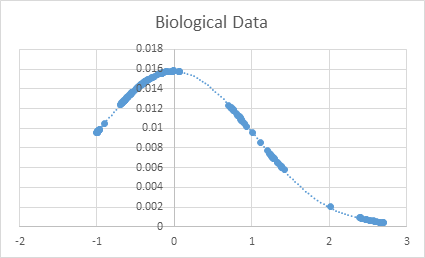
\includegraphics[height = 5cm]{Bio_Data}
	\caption[Aerial Biological Object Data]{Aerial Biological Object Data (Standard Normal Distribution)}
\end{table}

\begin{table}[H]
	\center 
	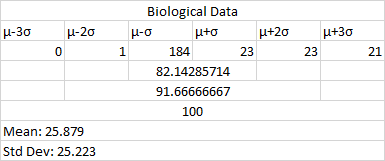
\includegraphics[height = 3cm]{Bio_Exp}
	\caption[Aerial Biological Object Standard Normal Distribution Interpretation]{Aerial Object Biological Data Interpretation (Standard Deviation Percentiles)}
\end{table}

\newpage

\begin{table}[H]
	\center 
	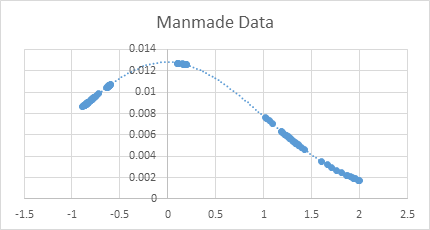
\includegraphics[height = 5cm]{Man_Data}
	\caption[Aerial Manmade Object Data]{Aerial Manmade Object Data (Standard Normal Distribution)}
\end{table}

\begin{table}[H]
	\center 
	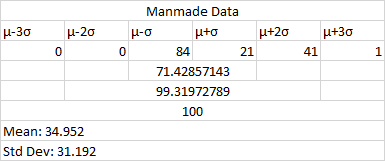
\includegraphics[height = 3cm]{Man_Exp}
	\caption[Aerial Manmade Object Standard Normal Distribution Interpretation]{Aerial Manmade Object Data Interpretation (Standard Deviation Percentiles)}
\end{table}

\indent The Heteroscedastic Paired T-test between the aerial biological and manmade objects' steady state ratios yielded a P-value of 0.001524.

\newpage

\begin{table}[H]
	\center 
	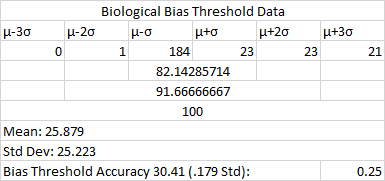
\includegraphics[height = 3cm]{Bio_Bias}
	\caption[Aerial Biological Object Bias Threshold Differentiation Accuracy]{Aerial Biological Object Bias Threshold Differentiation Accuracy (\%)}
\end{table}

\begin{table}[H]
	\center 
	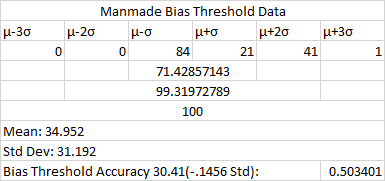
\includegraphics[height = 3cm]{Man_Bias}
	\caption[Aerial Manmade Object Bias Threshold Differentiation Accuracy]{Aerial Manmade Object Bias Threshold Differentiation Accuracy (\%)}
\end{table}

\indent The differentiation accuracy found in this study from the bias threshold in the two data sets yielded a 25\% accuracy rate for the aerial biological objects and 50.3% accuracy rate for the aerial manmade objects. 

\newpage